\lab{Algorithms}{Canonical Transformations}{Canonical Transformations}
\label{Ch:Canonical Transformations}

\objective{Understand Householder Transformations and Givens Rotations, and explore the reason that they are used in numerical computing.}

\section*{Unitary transformations}
{\bf TO DO} Explain the reason we use unitary transformations: Very numerically stable. (condition number of one)

Any unitary matrix can be thought of as a rigid reflection, a rigid rotation, or some combination of the two. For a unitary matrix $Q$, if $det(Q) = 1$, $Q$ is a rotation; if $det(Q) = -1$, $Q$ can be expressed as the composition of a reflection and a rotation.  In this section we explore these two types of unitary transformations and some of their applications.

\section*{Householder reflections}
A Householder reflection is a linear transformation $P: \mathbb{R}^n \rightarrow \mathbb{R}^n$ that reflects a vector $x$ about hyperplane. (See figure \ref{fig:Householder reflector}.) Recall that a hyperplane can be defined by a unit vector $v$ which is orthogonal to the hyperplane. As shown in the figure, $x - \langle v,x \rangle v$ is the projection of $x$ onto the hyperplane defined by $v$. (You should verify this geometrically.) However, to reflect \emph{across} the hyperplane, we must move twice as far; that is, $Px = x - 2\langle v,x \rangle v$. This can be written $Px = x - 2v(v^\ast x)$, so $P$ has matrix representation $P = I - 2vv^\ast$. Note that $P^\ast P = I$; thus $P$ is unitary.

\begin{figure}
\label{fig:Householder reflector}
	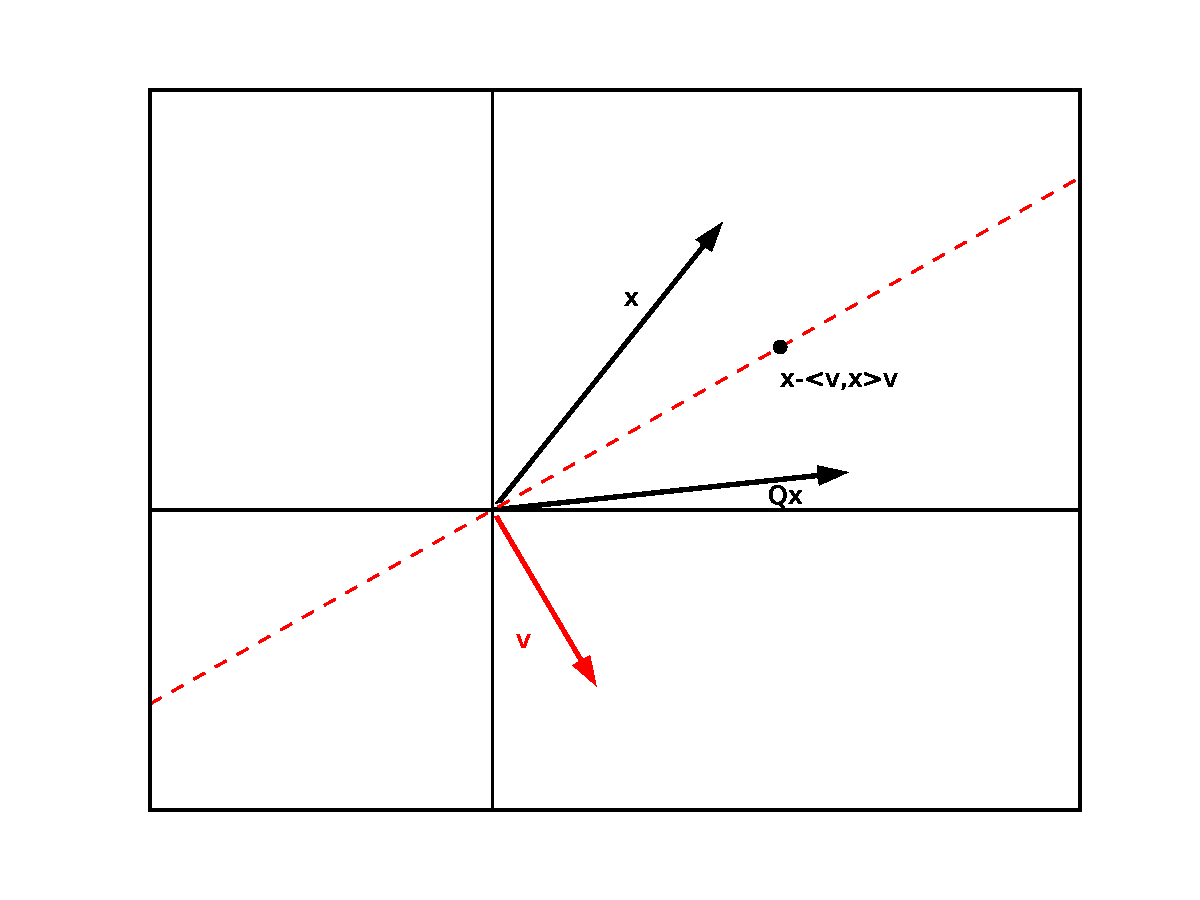
\includegraphics{fig1}
\end{figure}

\subsection*{Householder triangularization}
Consider the problem of computing the $QR$ decomposition of a matrix $A$. (Throughout this section, assume $A$ is real.) You've already learned the Gram-Schmidt and the Modified Gram-Schmidt algorithms for this problem. The $QR$ decomposition can also be computed using Householder triangularization. Gram-Schmidt and Modified Gram-Schmidt \emph{orthogonalize} $A$ by a series of \emph{triangular} transformations. Conversely, the Householder method \emph{triangularizes} $A$ by a series of \emph{orthogonal} transformations.

Let's demonstrate this method on a $4 \times 3$ matrix $A$. First we find a unitary transformation $Q_1$ that maps the first column of A into the range of $e_1$.

\def\mc#1{\multicolumn{1}{c|}{#1}}
\begin{equation*}
\begin{pmatrix}
\ast & \ast & \ast \\
\ast & \ast & \ast \\
\ast & \ast & \ast \\
\ast & \ast & \ast 
\end{pmatrix}
\underrightarrow{Q_1}
\begin{pmatrix}

\ast & \ast & \ast & \\ \cline{2-3}
\mc{0} & \ast & \mc{\ast}& \\
\mc{0} & \ast & \mc{\ast} & \\
\mc{0}& \ast & \mc{\ast} & \\ \cline{2-3}
\end{pmatrix}
\end{equation*}
Let $A_2$ be the boxed submatrix of $A$. Now find an orthogonal transformation $Q_2$ that maps the first column of $A_2$ into the range of $e_2$. 

\begin{equation*}
\begin{pmatrix}
\ast & \ast \\
\ast & \ast \\
\ast & \ast 
\end{pmatrix}
\underrightarrow{Q_2}
\begin{pmatrix}
\ast & \ast \\
0 & \ast \\
0 & \ast 
\end{pmatrix}
\end{equation*}
Similarly, $ \begin{pmatrix} \ast \\ \ast \end{pmatrix} \underrightarrow{Q_3} \begin{pmatrix} \ast \\ 0 \end{pmatrix} $. If we choose $Q_2$ and $Q_3$ so they don't ``mess with" the zeros we've already obtained, then we'll have $Q_3 Q_2 Q_1 A =$ 

\begin{equation*}
Q_3 Q_2 Q_1
\begin{pmatrix}
\ast & \ast & \ast \\
\ast & \ast & \ast \\
\ast & \ast & \ast \\
\ast & \ast & \ast \\
\end{pmatrix}
= Q_3 Q_2
\begin{pmatrix}
\ast & \ast & \ast \\
0 & \ast & \ast \\
0 & \ast & \ast \\
0 & \ast & \ast \\
\end{pmatrix}
= Q_3
\begin{pmatrix}
\ast & \ast & \ast \\
0 & \ast & \ast \\
0 & 0 & \ast \\
0 & 0 & \ast \\
\end{pmatrix}
= 
\begin{pmatrix}
\ast & \ast & \ast \\
0 & \ast & \ast \\
0 & 0 & \ast \\
0 & 0 & 0 \\
\end{pmatrix}
\end{equation*}
(Technically $Q_2$ and $Q_3$ act on the whole matrix and not just on the submatrices, so that $Q_i: \mathbb{R}^n \rightarrow \mathbb{R}^n$ for all $i$. $Q_2$ leaves the first row alone, and $Q_3$ leaves the first two rows alone.)

We've accomplished our goal, which was to triangularize $A$ using orthogonal transformations. But now, how do we find the $Q_i$ that do what we want? Using Householder reflections. 

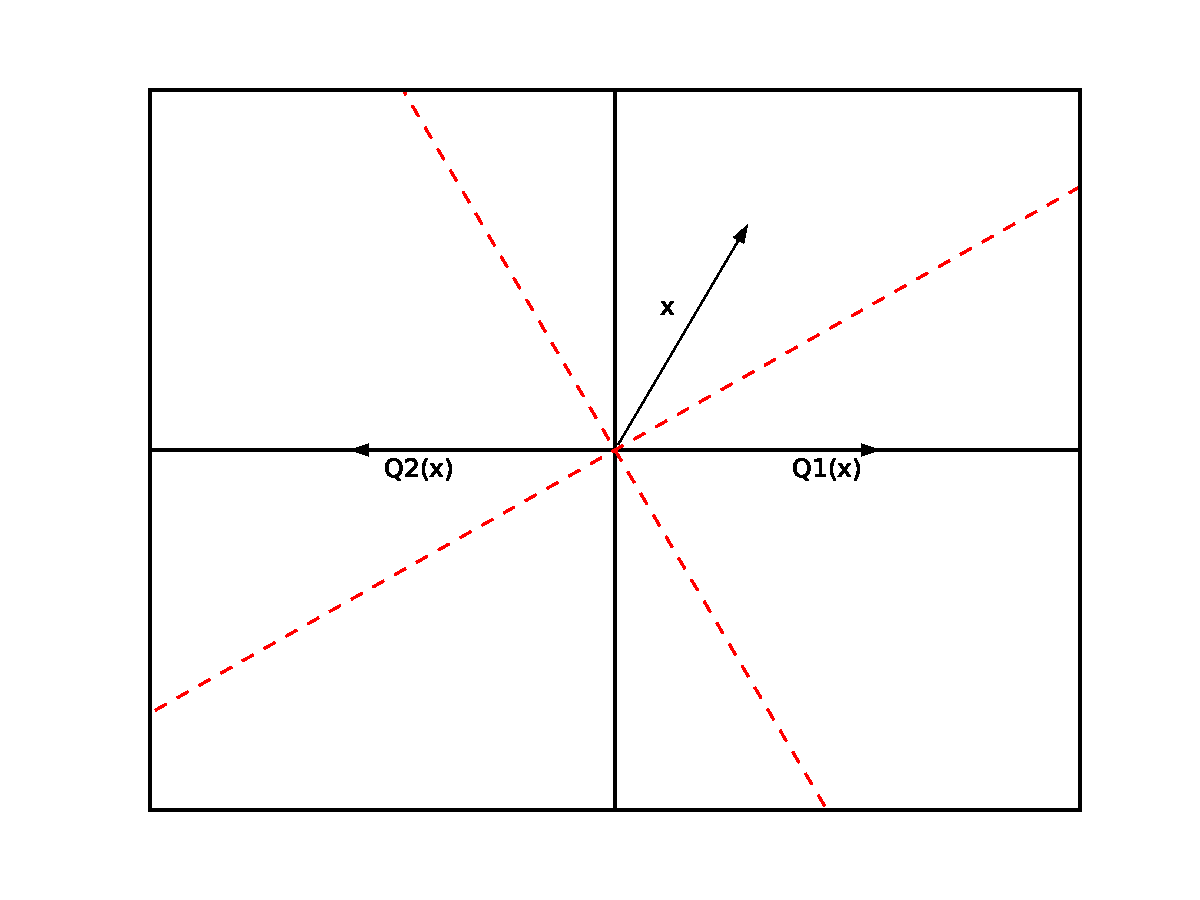
\includegraphics{fig2.pdf}

For example, to find $Q_1$, we choose the right hyperplane to reflect $x$ into the range of $e_1$. What is the right hyperplane? It turns out there are two hyperplanes that will work, as shown in Figure 2 *** reference figure***. (In the complex case, there are infinitely many such hyperplanes.) Between the two, the one that reflects $x$ further will be more numerically stable. This is the hyperplane perpendicular to $v = sign(x_1)\norm{x}e_1 + x$. This process is summarized in algorithm \ref{Alg:Householder triangularization}.


\begin{pseudo}{Householder triangularization}{A}
\label{Alg:Householder triangularization}
\FOR k = 1 \TO n\\
   x = A_{k:m,k}\\
   v_k = sign(x_1)\norm{x}_2 e_1 + x\\
   v_k = v_k / \norm{v_k}_2\\
   A_{k:m,k:n} = A_{k:m,k:n} - 2 v_k (v_k^\ast A_{k:m,k:n})
\end{pseudo}

This algorithm triangularizes $A$ and also generates a set of vectors $v_k$ that can be used to compute $Q$. However, we can avoid computing $Q$ directly by using the $v_k$ to compute $Qx$ for a given $x$, as indicated in algorithm \ref{Alg:Calculate Qx}


\begin{pseudo}{Calculate Qx}{x,v_1, \hdots , v_n}
\label{Alg:Calculate Qx}
\FOR k = n \DOWNTO 1\\
x_{k:m} = x_{k:m} - 2v_k(v_k^\ast x_{k:m})
\end{pseudo}

If we do want to generate $Q$, we simply calculate $Qe_i$ for $i = 1 \hdots m$.

\begin{problem}
Write a script using Householder reflections to find the QR decomposition of a matrix A.
\end{problem}

\subsection*{Stability of the Householder QR algorithm}


{\bf TO DO} Discuss forward/backward stability

Try the following in iPython.

\begin{lstlisting}
In [1]:  Q,X = linalg.qr(sp.rand(50,50)) #create a random orthogonal matrix:
In [2]:  R = sp.triu(sp.rand(50,50)) # create a random upper triangular matrix
In [3]:   A = sp.dot(Q,R) #Q and R are the exact QR decomposition of A
# use your Householder QR script to estimate Q and R:
In [4]:   Q1,R1 = householder.qr(A)
#now check the relative errors of Q1 and R1
In [5]:  linalg.norm(Q1-Q)/linalg.norm(Q)
Out [5]: 
\end{lstlisting}
Now check the relative errors of $Q_1$ and $R_1$.
\begin{lstlisting}

\end{lstlisting}


Householder QR factorization is more numerically stable than Gram-Schmidt or even Modified Gram-Schmidt (MGS). However, MGS is still useful for some types of iterative methods, because it finds the orthogonal basis one vector at a time instead of all at once (for example see Lab \ref{Ch:EigSolve}).

\subsection*{Upper Hessenberg Form}

An upper Hessenberg matrix is a square matrix with zeros below the first subdiagonal. Every complex \footnotemark $n \times n$ matrix $A$ can be written $A = Q^*HQ$ where $Q$ is unitary and $H$ is an upper Hessenberg matrix, called the Hessenberg form of $A$. Note the similarity of this decomposition to the Schur decomposition in Lab \ref{Ch:Jordan}. \footnotetext{It's okay if $A$ is real, as long as we allow $Q$ and $H$ to be complex.}

The Hessenberg decomposition can be computed using Householder reflections, in a process very similar to Householder triangularization. Let's demonstrate this process on a $5 \times 5$ matrix $A$. Note that $A=Q^*HQ$ is equivalent to $QAQ^* = H$; thus our strategy is to multiply $A$ on the right and left by a series of unitary matrices until it is in Hessenberg form. If we try the same $Q_1$ as in the first step of the Householder algorithm, then with $Q_1 A$ we introduce zeros in the first column of $A$. However, since we now have to multiply $Q_1 A$ on the left by $Q_1^*$, all those zeros are destroyed.
\[
\begin{array}{ccccc} 
\begin{pmatrix}
* & * & * & * & *\\
* & * & * & * & *\\
* & * & * & * & *\\
* & * & * & * & *\\
* & * & * & * & *\\
\end{pmatrix} 
&\underrightarrow{Q_1 \cdot }&
\begin{pmatrix}
* & * & * & * & *\\
0 & * & * & * & *\\
0 & * & * & * & *\\
0 & * & * & * & *\\
0 & * & * & * & *\\
\end{pmatrix} 
&\underrightarrow{\cdot Q_1^* }&
\begin{pmatrix}
* & * & * & * & *\\
* & * & * & * & *\\
* & * & * & * & *\\
* & * & * & * & *\\
* & * & * & * & *\\
\end{pmatrix} 
\\ 
A & & Q_1A & & Q_1 A Q_1^*
  \end{array}
\]
Instead, let's try starting with a different $Q_1$ that leaves the \emph{first} row alone and reflects the \emph{rest} of the rows into the range of $e_2$. This means that $Q_1^*$ leaves the first column alone.
\[
\begin{array}{ccccc} 
\begin{pmatrix}
* & * & * & * & *\\
* & * & * & * & *\\
* & * & * & * & *\\
* & * & * & * & *\\
* & * & * & * & *\\
\end{pmatrix} 
&\underrightarrow{Q_1 \cdot }&
\begin{pmatrix}
* & * & * & * & *\\
* & * & * & * & *\\
0 & * & * & * & *\\
0 & * & * & * & *\\
0 & * & * & * & *\\
\end{pmatrix} 
&\underrightarrow{\cdot Q_1^* }&
\begin{pmatrix}
* & * & * & * & *\\
* & * & * & * & *\\
0 & * & * & * & *\\
0 & * & * & * & *\\
0 & * & * & * & *\\
\end{pmatrix} 
\\ 
A & & Q_1A & & Q_1 A Q_1^*
  \end{array}
\]
We now iterate through the matrix until we obtain
\begin{equation*}
Q_3 Q_2 Q_1 A Q_1^* Q_2 ^* Q_3^* = 
\begin{pmatrix}
* & * & * & * & *\\
* & * & * & * & *\\
0 & * & * & * & *\\
0 & 0 & * & * & *\\
0 & 0 & 0 & * & *\\
\end{pmatrix} 
\end{equation*}

\begin{problem}
Write a script that transfers an input matrix to upper Hessenberg form. (Hint: Modify algorithm \ref{Alg:Householder triangularization} to obtain $H$, and modify algorithm \ref{Alg:Calculate Qx} to obtain $Q$.) We will use this technique in the eigenvalue lab later. {\bf TO DO} Do we need the unitary matrix as well?
\end{problem}

\section*{Givens rotations}

Givens rotations are not as fast as Householder for computing $QR$ in general. But they are very parallelizable, and are faster than Householder when $A$ is sparse.

\begin{problem}
Write a script that uses Givens rotations to do QR decomposition.
\end{problem}

\begin{problem} 
Compare the MGS, Householder, and Givens algorithms for $QR$ decomposition. Which is the fastest? Which is the most stable?
\end{problem}

%Sources: http://www.cs.unc.edu/~krishnas/eigen/node5.html
% http://en.wikipedia.org/wiki/Givens_rotation
%http://en.wikipedia.org/wiki/QR_decomposition
%	Note the Operation count: Householder is 2/3 n^3, MGS is 2 n^3
%http://en.wikipedia.org/wiki/QR_algorithm
%Applied Numerical methods using MATLAB by Yang has some code written for this
%http://www.math.kent.edu/~reichel/courses/intr.num.comp.2/lecture21/evmeth.pdf
%	These are eigenvalue algorithms explained carefully
%http://en.wikipedia.org/wiki/Householder_transformation
%Numerical Linear Algebra, by Lloyd N. Trefethen and David Bau III, Chapters 10 and 16

